\setcounter{footnote}{0}
\section{引言}\label{sec:1}

\subsection{Dirichlet $L$-值}\label{sec:1.1}

黎曼 $\zeta$ 函数之值 $\zeta(k)$ (其中 $k$ 为正整数), 
以及更一般的针对二次特征 $\chi$ 的 Dirichlet $L$-值
\[ L(k,\chi) = \sum_{n=1}^{\infty} \frac{\chi(n)}{n^k} \]
长期以来一直是数学家们关注的焦点.
假设 $\chi$ 是导体为 $D$ 的原始二次特征, 这里我们采用的约定是 $D$ 的符号即为 $\chi(-1)$ 的符号.
由 Euler \cite{Eul1735} 和 Dirichlet \cite{Dir1837} 的开创性工作
(甚至早在 $D = -4$ 且 $k = 1$ 的特殊情况下 \cite{Roy90}), 我们知道, 对于正整数 $k$:
\begin{equation}\label{eq:1.1.1}
L(k,\chi) \in \begin{cases} \pi^k \cdot \sqrt{D} \cdot \mathbf{Q}^{\times}, & \text{当 } k \text{ 为偶数且 } \chi(-1) = 1, \\ \pi^k \cdot \sqrt{-D} \cdot \mathbf{Q}^{\times}, & \text{当 } k \text{ 为奇数且 } \chi(-1) = -1, \\ \sqrt{D} \log \left( |\overline{\mathbf{Q}}^{\times}| \setminus \{1\} \right), & \text{当 } k = 1, \ \chi(-1) = 1, \text{ 且 } D \neq 1. \end{cases}
\end{equation}

结合 Lindemann 定理 \cite{Lin1882} (该定理证明了 $\pi$ 是超越数) 
以及 Weierstrass 对其在代数数(非 $0$ 或 $1$)的自然对数超越性上的推广 \cite{Wei1885}, 
我们知道所有这些值都是超越数.
然而, 剩下的 $L$-值我们对其知之甚少.
事实上, 自 Weierstrass 的工作 \cite{Wei1885} 以来近 $140$ 年的时间里, 
仅有唯一一个更具体的数值 $L(k, \chi)$ 被证明是无理数, 
即 Ap{\'e}ry 在 $1978$ 年出人意料地证明了 $\zeta(3)$ 是无理数 \cite{Ape79}\cite{vdP79}\cite{Coh78}.
在本文中, 我们确立了一个新的 $L$-值 $L(k, \chi)$ 的无理数性质;
在某种意义上, 这是最``简单''的未决情形, 对应于 $k = 2$ 且特征为具有最小导体的 $\chi = \chi_{-3}$.

\begin{maintheorem}\label{thm:A}
周期
\begin{align*}
L(2,\chi_{-3}) &= \sum_{n=0}^{\infty} \left( \frac{1}{(3n+1)^2} - \frac{1}{(3n+2)^2} \right) = 0.7813024128964862968 \dots \\
&= \iint_{1 \ge y \ge x \ge 0} \frac{dxdy}{y(1+x+x^2)} = -\int_0^1 \frac{\log(x)dx}{1+x+x^2}
\end{align*}
是无理数.
更一般地, $1$, $\pi^2$, $L(2, \chi_{-3})$ 这三个周期在 $\mathbf{Q}$ 上是线性无关的.
\end{maintheorem}

上述公式展示了 $L(2, \chi_{-3})$ 作为一个 Kontsevich--Zagier 意义上的周期 \cite{KZ01}.
对于 $L(2, \chi_{-3})$, 还存在许多其他更复杂的积分或无穷级数表达式,
例如, 以下超几何类型的和 (\cite[§3]{HPHP11}):
\[ L(2,\chi_{-3}) = \frac{1}{27} \sum_{n=1}^{\infty} \frac{(4-15n)(-27)^n}{n^3 \binom{2n}{n}^2 \binom{3n}{n}}, \]
或者更巧合地, 可以用杨辉三角中大于一的项的倒数平方和来表示 \cite{Sta23}:
\[ L(2,\chi_{-3}) = -\frac{1}{3} + \sum_{n>m>0} \frac{1}{\binom{n}{m}^2}. \]

常数 $3\sqrt{3} L(2,\chi_{-3})/4 = \mathrm{Im}(\mathrm{Li}_2(e^{\pi i/3})) = \frac{3}{2} \cdot \mathrm{Im}(\mathrm{Li}_2(e^{2\pi i/3})) = 1.014941\dots$ 
是正规理想双曲四面体(具有最大体积的四面体)的体积,
同时也是具有极小体积的非紧双曲流形 \cite{Ada87} (即 Gieseking 流形, 其可定向双覆盖是八字结的余集 \cite{Thu97}) 的体积.
证明双曲 $3$-维流形的体积在有理数上不都相关是一个未决问题 (参见 \cite[Problem 23]{Thu82}, 以及 \cite{Mil82}\cite{Mil83}).
虽然我们的结果对这个问题没有直接的影响, 但它是第一个与这些体积的算术性质建立联系的无条件结果.
$L(2, \chi_{-3})$ 的另一个出现是在 Smyth 公式中 \cite[Prop. 3.4]{BZ20}:
\begin{equation}\label{eq:1.1.2}
\frac{3\sqrt{3}}{4\pi}L(2,\chi_{-3}) = m(1+x+y) := \int_0^1 \int_0^1 \log|1 + e^{2\pi i s} + e^{2\pi i t}| \, ds \, dt
\end{equation}
该公式将 $L(2, \chi_{-3})$ 关联到最简单的本质上是二元的多项式 $1+x+y$ 的 Mahler 测度,
或者等价地用代数几何和 Arakelov 几何的语言来说 \cite{Phi91}\cite{BGS94}, 
关联到线性代数环面 $\mathbf{G}_m^2$ 的子簇 $1+x+y=0$ 的正则高度.
不幸的是, 虽然整系数一元多项式的非零 Mahler 测度由 Hermite--Lindemann--Weierstrass 定理 \cite{Her1874}\cite{Lin1882}\cite{Wei1885} 已知是超越数, 
但我们的结果对任何此类正则高度的猜想无理数性质没有直接关系!
(顺便提一句, 我们也证明了有理系数二元多项式 $(1+x+y)^4/3$ 的 Mahler 测度的无理数性质, 这并不是一个正则高度. 这可见于定理 2.11.17.)

\autoref{thm:A} 的一个直接推论是以下``三伽马 (trigamma)''函数 $\psi_1(z) = \sum_{n=0}^{\infty} \frac{1}{(z+n)^2} = \zeta(2,z)$ 之值的无理数性质:

\begin{maincorollary}\label{cor:B}
以下数值是无理数:
\begin{align*}
\frac{1}{1^2} + \frac{1}{4^2} + \frac{1}{7^2} + \frac{1}{10^2} + \dots &= \frac{L(2, \chi_{-3})}{2} + \frac{2\pi^2}{27}, \\
\frac{1}{2^2} + \frac{1}{5^2} + \frac{1}{8^2} + \frac{1}{11^2} + \dots &= -\frac{L(2, \chi_{-3})}{2} + \frac{2\pi^2}{27}, \\
\frac{1}{1^2} + \frac{1}{7^2} + \frac{1}{13^2} + \frac{1}{19^2} + \dots &= \frac{5L(2, \chi_{-3})}{8} + \frac{\pi^2}{18}, \\
\frac{1}{5^2} + \frac{1}{11^2} + \frac{1}{17^2} + \frac{1}{23^2} + \dots &= -\frac{5L(2, \chi_{-3})}{8} + \frac{\pi^2}{18}.
\end{align*}
\end{maincorollary}

注意到由于 $\psi_1(x+1) - \psi_1(x) + 1/x^2 = 0$, 
由 \autoref{thm:A} 
(结合 $\psi_1(1) = \pi^2/6$ 且 $\psi_1(1/2) = \pi^2/2$)
同样可以推导出 $\psi_1(n/6)$ 对于任何 $n \in \mathbb{N}_{>0}$ 都是无理数.
自 Legendre 于 $1794$ 年证明 $\pi^2$ 是无理数以来 \cite{Leg1794}, 这些是关于 $\psi_1$ 的首批新的无理数结果!

作为完全相同的论证的另一个应用, 我们也证明了关于两个对数的某些乘积的如下无理数结果 (见第 14 节中的定理 14.0.1).

\begin{maintheorem}\label{thm:C}
设 $m, n \in \mathbb{Z} \setminus \{-1, 0\}$ 是整数, 满足 
\[ \left| \frac{m}{n} - 1 \right| < \frac{1}{10^6}. \]
则
\[ \log \left( 1 + \frac{1}{m} \right) \log \left( 1 + \frac{1}{n} \right) \]
是无理数. 
此外, 当 $m \neq n$ 时, 以下数值在 $\mathbf{Q}$ 上是线性无关的:
\[ 1, \quad \log\left(1+\frac{1}{m}\right), \quad \log\left(1+\frac{1}{n}\right), \quad \log\left(1+\frac{1}{m}\right)\log\left(1+\frac{1}{n}\right). \]
\end{maintheorem}

\subsection{与 Ap{\'e}ry 工作的对比}\label{sec:1.2}

Ap{\'e}ry 的证明 \cite{vdP79} 包含寻找一个显式的有理数逼近序列, 该序列``足够快''地收敛到 $\zeta(3)$ 以证明 $\zeta(3)$ 是无理数.
自 Ap{\'e}ry 的结果发表以来, 人们付出了巨大努力来寻找类似的序列, 以证明除 \eqref{eq:1.1.1} 形式以外的其他 $L$-值 $L(k, \chi)$ 的无理数性质.
不幸的是, 尽管付出了艰苦的努力, 依然没有找到这样的序列.\footnote{一个与特定 $L$-值的无理数性质无直接关系的重要步骤是 Ball 和 Rivoal 的定理 \cite{Riv00}\cite{BR01}, 该定理证明了无穷多个奇数 $\zeta$ 值是无理数. Zudilin 的一个精细化结果 \cite{Zud01} 证明了 $\zeta(5)$, $\zeta(7)$, $\zeta(9)$ 和 $\zeta(11)$ 这四个值中至少有一个是无理数.}
特别是, 在本文中, 我们并没有(直接)找到任何新的收敛到 $L(2, \chi_{-3})$ 的级数.
相反, 我们展示了如何利用超越数论和复分析的方法, 以一种更微妙的方式利用已知的逼近级数(由 Ap{\'e}ry 和其他人发现)的算术特征.

为了引入我们的主要思想, 我们首先进行阐述, 然后对 Ap{\'e}ry 证明的一些关键特征进行重新表述.
首先要指出的是, Ap{\'e}ry 的证明使用了很少的数论知识;
事实上, 唯一的数论输入是素数定理的弱形式 and 以下初等引理:

\begin{lemma}\label{lem:1.2.1}
如果存在一个 $\delta > 0$ 以及一个有理数序列 $p_n/q_n \neq \beta$ 且当 $q_n \to \infty$ 时满足:
\[ \left|\beta - \frac{p_n}{q_n}\right| < \frac{1}{q_n^{1+\delta}} \qquad n = 1, 2, \dots, \]
则 $\beta$ 是无理数.
\end{lemma}

即使在更弱的假设下, 即当 \(\lvert\beta - p_n/q_n\rvert = o(1/q_n)\) 时, 该引理依然成立.
Ap{\'e}ry 写下了一对幂级数 \(A(x), B(x) \in \mathbf{Q}[x]\) 以及它们的线性组合:
\begin{equation*}
  P(x) = B(x) - \zeta(3)A(x) = \sum_{n=0}^{\infty} x^n (b_{n} - \zeta(3)a_{n}).
\end{equation*}
其中的系数 \(a_n\) 和 \(b_n\) 是有理数, 更准确地说:
\begin{equation*}
  a_{n} \in \mathbf{Z}, \qquad {[1, 2, 3, \dots, n]}^3 b_{n} \in \mathbf{Z}.
\end{equation*}
这里以及在我们的整篇论文中, 我们遵循惯用记号 $[1, 2, 3, \dots, n]$ 来表示前 $n$ 个整数的最小公倍数.
素数定理决定了这些分母的增长率:
\[ \log[1, 2, 3, \dots, n] = n + o(n). \]
与此同时, Ap{\'e}ry 证明了 $A(x)$ (和 $B(x)$) 的收敛半径为 $(\sqrt{2}-1)^4$, 
而 $P(x)$ 的收敛半径恰好为 $(\sqrt{2}+1)^4$.
现在我们可以利用不等式
\begin{equation}\label{eq:1.2.2}
4\log(\sqrt{2}+1) > 3
\end{equation}
来推导, 结合 \autoref{lem:1.2.1} 并且令 $p_n/q_n = b_n/a_n$ 且
\[ \delta = \frac{4\log(\sqrt{2}+1) - 3}{4\log(\sqrt{2}+1) + 3}, \]
便可得到 $\zeta(3) \notin \mathbf{Q}$.

在很多其他情况下, 人们也可以构造类似风格的函数 $A(x), B(x)$, 使得特定的线性组合 $P(x) = B(x) - \eta A(x)$ 具有额外的收敛性质, 
其中 $\eta = L(k,\chi)$ 是由这种性质唯一刻画的复数.
但是类似于 \eqref{eq:1.2.2} 的不等式似乎总是无法成立\footnote{除了 Ap{\'e}ry 自身发现的具有 $\eta = \zeta(2)$ 的一个显著例子外.}, 
因而无法对相应的 $L$-值的算术性质得出任何结论.
(关于 Ap{\'e}ry 所考虑的形式序列的一个特别有趣的探讨, 见 \cite{Zag09}.
在我们证明 \autoref{thm:A} 的过程中, 我们将核心使用 Zagier 在其探索中(重新)发现的一些级数.)

我们研究的出发点是, 即使当 \eqref{eq:1.2.2} 的类似物像通常那样不成立时, 这些构造中出现的函数 $P(x)$ 也具有以前未被利用的更深层的结构.
Ap{\'e}ry 的函数 $A(x)$ and $B(x)$ 满足一个在 $\mathbf{Z}[x]$ 中具有系数的线性常微分方程 (ODE),
该方程仅在 $x=0, \infty$ 和 $(\sqrt{2}\pm 1)^4$ 处具有(正则)奇点.
函数 $P(x)$ 是作为该 ODE 满足在 $0$ 处全纯的二维解空间中的唯一(在乘上一个常数意义下)线性组合而出现的,
它同时还具有在 $(\sqrt{2}-1)^4$ 处全纯的额外性质.
这意味着 $P(x)$ 不仅在半径为 $(\sqrt{2}+1)^4$ 的圆盘上是全纯的, 
而且可以解析开拓为在整个 $\mathbf{C} \setminus [(\sqrt{2}+1)^4, \infty)$ 上的全纯函数,
或者 (更符合我们最终的目的, 但在引言中不那么重要) 解析开拓为在
\[ \mathbf{P}^1 \setminus \{0, (\sqrt{2}-1)^4, (\sqrt{2}+1)^4, \infty\} \]
的万有覆盖上的全纯函数, 它在 $x = 0$ 处全纯, 并且在跨越第一个奇点 $(\sqrt{2} - 1)^4$ 后是超收敛 (overconvergent) 的.
Ap{\'e}ry 所使用的全部性质仅仅是 $P(x)$ 在半径为 $(\sqrt{2} + 1)^4$ 的圆盘上全纯.

现在想象一个类似的情形, 其中 $A(x)$ 和 $B(x)$ 是在一个 ODE\footnote{与本文中的情况一致, 我们指的总是 $\mathbf{Q}(x)$ 上的线性 ODE.} 在 $x=0$ 处全纯的解, 
该方程在 $0, \infty$ 和一对实数 $0 < \alpha < \beta$ 处具有正则奇点,
并且 $P(x) = A(x) - \eta B(x)$ 是一个在线性组合, 它在 $\alpha$ 处也是全纯的, 
但是其解析开拓在 $\beta$ 处具有奇点, 并且在 $x=\beta$ 处不能解析开拓为亚纯函数.
但是现在假设——考虑到 $a_n$ 和 $b_n$ 的分母——常数 $\beta$ 不够大, 
不足以说明相应的收敛子 $p_n/q_n$ 满足 \autoref{lem:1.2.1}.
是否有办法利用以下事实: $P(x)$ 不仅在半径为 $\beta$ 的圆盘上是全纯函数, 
而且可以延伸为在 $\mathbf{C} \setminus [\beta, \infty)$ 以及在 $\mathbf{P}^1 \setminus \{0, \alpha, \beta, \infty\}$ 的万有覆盖上的全纯函数?

为了使问题更简单 (事实上是过于简单了——我们将回到分母的必要性问题上), 
让我们暂时假设 $a_n$ 和 $b_n$ 实际上是整数.
为了通过 \autoref{lem:1.2.1} 运行 Ap{\'e}ry 的证明方案, 在这种情况下只需满足 $\beta > 1$ 即可.
在这种情况下, \autoref{lem:1.2.1} 具有以下交替表述:

\begin{lemma}[Simple Lemma]\label{lem:1.2.3}
一个在 $\mathbf{Z}[\![x]\!]$ 中的整系数幂级数, 如果定义了在半径为 $R > 1$ 的圆盘 $|x| < R$ 上的全纯函数, 那么它必定是一个多项式.
\end{lemma}

在我们的运行示例中, 如果 $\beta < 1$, 我们不能从 \autoref{lem:1.2.3} 推导出任何结论, 
但我们仍然可以推导出 $P(x)$ 在 $\mathbf{C} \setminus [\beta, \infty)$ 上是全纯的.
有一个专门研究 \autoref{lem:1.2.3} 的更微妙推广的完整学科, 
始于 Borel--P{\'o}lya 定理 (参见 \cite[Chapter 5]{Ami75}), 
它允许人们从比仅仅在足够大半径的圆盘上收敛更弱的解析假设中得出关于 $P(x) \in \mathbf{Z}[\![x]\!]$ 的结论.
我们现在回顾这个定理的一个特例.
如果 $\Omega \subset \mathbf{C}$ 是一个包含 $0$ 的单连通开区域, 
那么根据黎曼映射定理, 存在一个双全纯映射 $\varphi : \mathbf{D} \to \Omega$, 满足 $\varphi(0) = 0$.
映射 $\varphi$ 在保持 $0$ 不动的单位圆盘的双全纯映射下是唯一的, 这些映射均由旋转给出.
特别是, 不变量 $|\varphi'(0)|$ 不依赖于 $\varphi$ 的选择, 
并且(根据定义)等于 $\Omega$ 在 $0$ 处的共形半径 $\rho(\Omega, 0)$.
圆盘 $\mathbf{D}_R = D(0, R)$ 的共形半径等于 $R$ (通过映射 $\varphi(z) = Rz$), 
但是任何其他 $\Omega$ 的共形半径都严格大于包含在 $\Omega$ 中且以 $z = 0$ 为圆心的最大圆盘的半径.
我们有:

\begin{theorem}[Borel--P{\'o}lya, \cite{Pol1923}]\label{thm:1.2.4}
一个在 $\mathbf{Z}[\![x]\!]$ 中的幂级数 $P(x)$, 
如果解析开拓到包含 $0$ 且共形半径 $\rho(\Omega, 0) = |\varphi'(0)| > 1$ 的单连通开区域 $0 \in \Omega \subset \mathbf{C}$, 
则它必然是一个有理函数: $P(x) \in \mathbf{Q}(x)$.
\end{theorem}

例如, 双全纯映射
\[ \varphi: \mathbf{D} \to \mathbf{C} \setminus [\beta, \infty), \quad z \mapsto \frac{4\beta z}{(1+z)^2} \]
表明 $\mathbf{C} \setminus [\beta, \infty)$ 具有共形半径 $|\varphi'(0)| = 4\beta$.
因此, 从我们上面设想的例子中, 一旦 $4\beta > 1$, 
便可根据 \autoref{thm:1.2.4} 推导出 $P(x)$ 是一个有理函数, 
这与 $P(x)$ 在 $\beta$ 处不是亚纯的假设相矛盾, 并暗示 $\eta$ 是无理数.
这显然是对条件 $\beta > 1$ 的改进.
(关于 P{\'o}lya 定理这一特例的基本思想在引言末尾的 \autoref{rem:1.2.5} 中有简要介绍.)

甚至在 \autoref{thm:1.2.4} 之外 (正如我们将在下文\autoref{sec:2}中所讨论的), 
还有 Andr{\'e} 等人的代数性定理, 它们具有更弱的高度假设, 
允许人们推导出 $P(x)$ 在 $\mathbf{Q}(x)$ 上是代数的 (参见 \cite{And04}\cite{And89}\cite{CDT21}), 
这在实践中对于任何特定的 $P(x)$ 通常可以直接排除.

我们论文的主要精力在于调整和磨练 Borel, P{\'o}lya 和 Andr{\'e} 的方法, 以适应 Ap{\'e}ry 无理数证明的语境.
代数性判据本身并不适用, 
因为与 Ap{\'e}ry 风格证明相关的幂级数 $A(x)$ and $B(x)$ 从未(同时)具有整系数.
事实上, 当引入分母时 (即使是某种受控的分母), 代数性就不再是需要考虑的合适性质了.
首先, 艾森斯坦定理 \cite[§11.4]{BG06} 指出, 
任何在 $\mathbf{Q}(x) \cap \mathbf{Q}[\![x]\!]$ 中的代数函数的幂级数展开对于某些 $S \in \mathbf{N}_{>0}$ 具有 $\mathbf{Z}[1/S]$ 系数.
但从 Borel 定理(及其变体)的各种证明的角度来看, 
如果 $P(x) \in \mathbf{Z}[\![x]\!]$, 那么它的所有幂也是如此; 
但是如果 $P(x)$ 具有分母, 那么 $P(x)$ 的幂通常具有更糟糕的分母.
一个需要牢记的例子是
\[ -\log(1-x) = \sum_{n=1}^{\infty} \frac{x^n}{n}. \]
该函数具有如下性质: 乘以 $[1, 2, 3, \dots, n]$ (其数量级为 $e^n$) 可以同时清除前 $n$ 个系数的分母.
但是为了清除 $\log^m(1-x)$ 的前 $n$ 个系数的分母, 必须乘以数量级为
\[ [1,2,\ldots,n]\times[1,\ldots,n/2]\times\cdots\times[1,\ldots,n/m]=\exp\left(n\left(1+\frac{1}{2}+\ldots+\frac{1}{m}\right)+o(n)\right) \]
的分母.
在本文中, 对于 $b \in \mathbf{R}^{>0}$, 记号 $[1, 2, 3, \dots, bn]$ 指的是 $[1, 2, 3, \dots, \lfloor bn \rfloor]$.
另一方面, 微分确实保持了受控分母增长的性质.
因此, 与其期望得到一个代数性定理, 不如期望得到一个算术 holonomy 边界 (arithmetic holonomy bound), 
即限制由具有特定分母增长和解析性质且在微分下闭合的函数所生成的 $\mathbf{Q}(x)$-向量空间的维度.
这特别意味着, 在适当推广的 Borel--P{\'o}lya 条件下, 
解是 Siegel 意义上的 $G$-函数 (参见 \cite{Zan14} 和 \cite[§VIII.1]{DGS94}, 亦见定义 15.1.1).
此外, 人们可以指望对该 $G$-函数的阶(即由 $G$ 及其导数生成的 $\mathbf{Q}(x)$-模的秩)给出一个足够好的显式边界, 
这在给定情况下与某个显式逼近函数 $P(x) = B(x) - \eta A(x)$ 的结构相矛盾.
当做到这一点时, 最终的矛盾在于假设 $P(x) \in \mathbf{Q}[x]$, 即 $\eta \in \mathbf{Q}$.

这些算术 holonomy 边界最终是本文的主要关注点, 我们将在下文\autoref{sec:2}中对其进行详细介绍.

\begin{remark}\label{rem:1.2.5}
在一个非常特殊的情况下, Zudilin \cite{Zud17} 先前已经提出了这方面的一个暗示
(虽然没有应用到新的无理数证明中), 
他孤立了线性形式 $c_n = b_n - \eta a_n$ 上的一个条件, 
该条件暗示了生成函数 $P(x) = \sum_{n=0}^{\infty} c_n x^n$ 解析开拓到割平面 $\mathbb{C} \setminus [\beta, \infty)$.
虽然 Ap{\'e}ry 对收敛半径的使用集中在系数 $c_n$ 的衰减率 $\beta^{-n+o(n)}$ 上, 
但 Zudilin 强调了 Hankel 行列式序列 $\det(c_{i+j})_{i,j=0}^n$ 改进的衰减率 $(4\beta)^{-n^2+o(n^2)}$;
这确实是 $P(x)$ 在 $\mathbb{C} \setminus [\beta, \infty)$ 上的解析性的一个著名推论 \cite{Pol28}\cite{Pom69}.
在 $\beta > 1/4$ 的情况下, 后者实际上与 $\Omega = \mathbb{C} \setminus [\beta, \infty)$ 上的 \autoref{thm:1.2.4} 证明密切相关:
如果所有 $c_n \in \mathbb{Z}$, 则 Hankel 行列式也是有理整数, 
因此如果它们以小于一的指数速率衰减, 它们将从某一点开始消失, 
这最终意味着根据 Kronecker 的有理判定判据有 $P(x) \in \mathbb{Q}(x)$.
在 $c_n \in \mathbb{Q}$ 的情况下量化 Hankel 行列式的分母同样可以得出 Zudilin 关于 $\eta \notin \mathbb{Q}$ 的行列式判据.
参见第 2.7.7 节了解更精确的表述和推广.\end{remark}

\begin{remark}\label{rem:1.2.6}
我们认为, 本文的读者可能包括不熟悉我们先前论文 \cite{CDT21} 的细节或更广泛的双廷逼近分析方法的数学家.
冒着打断论述连贯性的风险, 我们在整篇论文中加入了许多被称为``基本注记''的阐释性段落, 
旨在帮助那些不熟悉这些内容的读者理清思路; 专家完全可以略过这些内容.\end{remark}

\begin{remark}[符号注记]\label{rem:1.2.7}
我们将使用 $\mathbf{N} = \{0, 1, 2, \dots\}$ 来表示包含零的自然数, 
并用 $\mathbf{N}_{>0}$ 来表示正整数.
根据上下文, $\mathbf{P}^1$ 将表示同构于 $\operatorname{Proj} \mathbf{Z}[T_0, T_1]$ 的方案 (即 $\mathbf{Z}$ 上的射影直线), 
或其 $\mathbf{C}$ 值点的复流形 $\mathbf{P}^1(\mathbf{C})$ 
(即共形球, 坐标为 $z := T_0/T_1$, 在其他地方通常表示为 $\widehat{\mathbf{C}}$ 或 $\mathbb{CP}^1$).
类似的双重含义也适用于模叠 $Y_0(2)$ 和 $Y(2)$.
在相关坐标(在上下文中总是很清楚, 但最常用 $z$ 表示)中半径为 $R \in (0,\infty]$ 的复圆盘 $D(0,R)$ 将用 $\mathbf{D}_R$ 表示, 
并且我们将写 $\mathbf{D} := \mathbf{D}_1$ 来表示单位半径圆盘, 并用 $\overline{\mathbf{D}}$ 表示其在 $\mathbf{C}$ 中的闭包.
单位圆 $\partial \overline{\mathbf{D}} = \{e^{2\pi i\theta} : \theta \in [0,1]\}$ 被记为 **T**, 其一致测度 $d\theta$ 被记为 $\mu_{\text{Haar}}$.
对于一个连通复流形 $M$, 我们将分别用 $\mathcal{O}(M)$ 和 $\mathcal{M}(M)$ 来表示全纯函数环和亚纯函数域.
记号 $\mathcal{O}(\overline{\mathbf{D}})$ 和 $\mathcal{M}(\overline{\mathbf{D}})$ 用于闭单位圆盘 $\overline{\mathbf{D}} \subset \mathbf{C}$ 的某些未指定开邻域上的相应函数.
在本文中, 我们通常对属于上半平面 $\mathbf{H}$ 的 $\tau$ 写 $q := e^{\pi i \tau}$, 
尽管我们偶尔也会写 $q = e^{2\pi i \tau}$.
(如 \cite{CDT21} 中所述, 这是历史约定迫使我们这样做的, 但除非另有说明, 我们总是使用第一种选择.)
通过一个轻微且无害的记号滥用, 模 $\lambda$ 函数
\begin{equation}\label{eq:1.2.8}
\lambda(q) := \frac{\left(\sum_{n \in 1+2\mathbf{Z}} q^{n^2/4}\right)^4}{\left(\sum_{n \in 2\mathbf{Z}} q^{n^2/4}\right)^4} = 16q \prod_{n=1}^{\infty} \left(\frac{1+q^{2n}}{1+q^{2n-1}}\right)^8 : \mathbf{H} \to \mathbf{C} \setminus \{0,1\}, \ \{q=0\} \mapsto 0
\end{equation}
将写在尖点填充坐标 $q \in \mathbf{D} := \{|q| < 1\}$ 中, 而不是 $\tau = \log(q)/(\pi i)$.
字母 $e$ 通常保留给 Euler 常数 $e \approx 2.718281$.
最后, 我们通过采用对于集合 $X$ 的任何子集 $A$ 和 $B$ 写作 $X \setminus \{A, B\} := X \setminus (A \cup B)$ 的约定, 承认了一个轻微的记号滥用.\end{remark}

\subsection{通往定理 A 和 C 的路径以及论文概述}\label{sec:1.3}

以下导引图 (\autoref{fig:1.3.0}) 简要给出了我们论文的逻辑结构.
在这里, 双虚线表示通往定理 A 和 C 有两条交替路径, 
要么通过第 6 节 (通过多元方法, 基于测度集中), 
要么通过第 7 节 (通过单变量方法, 基于某些 Arakelov 理论和 Bost 在评估高度上的不等式).
我们还略去了附录 B, 它与第 7 节关系最密切 (尽管两个方向之间没有依赖关系).
如果我们把自己限制在定理 A 的最短证明上, 可能会有一些(微小的)节省.
然而, 考虑到未来的发展和应用, 我们觉得最好把所有这些新想法都包括进来.
在许多方面, 这反映了我们先前论文 \cite{CDT21} 的经验, 该论文包含了主 holonomy 定理的三个证明.
那篇论文的一位审稿人曾建议删除该定理的一个特定证明, 其思想随后被证明对本文的进展至关重要.

我们现在非常简要地概述本论文.
第 2 节主要是介绍性的, 尽管第 2.5--2.11 节给出了我们主要结果的基本形式(这些结果要到第 6 节才会得到证明)以及一些应用,
第 2.12--2.13 节概述了我们证明 holonomy 边界的方法, 
随后在第 3 节中给出了详细介绍, 引入了函数超越理论的元素.
在第 3 节中, 我们还包括了对相关材料在适当历史背景下的进一步阐述, 旨在帮助读者将我们的想法放在更广泛的背景中.
在第 4 节中, 我们收集了关于高维大偏差和测度集中现象的一些基本事实.
在第 5 节中, 我们引入了这样一个想法(鉴于第 2 节的讨论, 这可能有些违反直觉): 尽管引入了新的分母, 但对我们的假定函数进行积分有时是有用的.
还包括了与积分引起的额外分母相关的一些技术计算, 这些计算遵循素数定理.
在第 6 节中, 我们证明了我们的第一个主 holonomy 边界定理 6.0.2.
在第 7 节中, 基于 Bost 和 Charles 的工作 \cite{BC22}, 
我们利用 Bost 的斜率方法框架证明了我们的第二个主 holonomy 边界 (或者更确切地说, 是几个密切相关的边界).
特别是, 定理 7.0.1 本质上是 \cite{BC22} 中结合我们在第 6 节中对分母的处理所得到的边界;
定理 7.1.6 是利用一个生长特征函数的凸性对定理 7.0.1 的进一步改进, 
该函数与 Bost--Charles 边界密切相关, 且其行为类似于 Nevanlinna 特征函数.
在第 8 节中, 我们统一了第 6--7 节的方法, 
并着眼于未来的应用, 得到了本文中最尖锐的 holonomy 边界.
在第 9--12 节中, 我们重新讨论了特定的模板(分母类型和奇点固定的情况), 
以便为将我们的 holonomy 边界应用到我们主要的无理数结果中做好准备.
在第 9 节中, 我们利用模曲线映射 $Y(2) \to Y_0(2)$ 
来关联 $\mathbf{P}^1 \setminus \{0, 1, \infty\}$ 和 $\mathbf{P}^1 \setminus \{0, 4, \infty\}$ 上的两个模板.
在第 10 节中, 我们讨论了 $\mathbf{P}^1 \setminus \{0,1,\infty\}$ 上的某些具有简单分母类型的 $G$-函数,
并且在第 11 节中, 我们引入了在 \cite{Zag09} 中出现的特定局部系统, 
这些系统基于 $1, \pi^2$ 和 $L(2, \chi_{-3})$ 的假设线性相关性, 产生更多的 $G$-函数.
第 12 节致力于证明所有这些函数在 $\mathbf{C}(x)$ 上的线性无关性.
在第 13 节和第 14 节中, 我们分别利用一些在附录 A 中有详细解释的显式计算, 
给出了定理 A 和 C 的证明.

\addtocounter{equation}{-1}
\begin{figure}[!htbp]
  \centering
  % 拷贝后的原图路径为 assets/fig/CDT_L_2026_leitfaden.jpeg 
  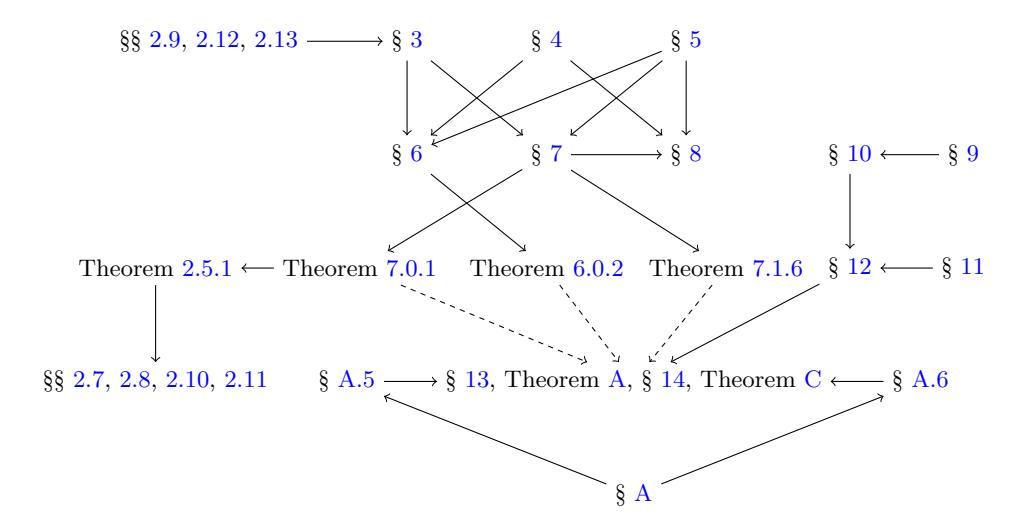
\includegraphics[width=0.6\textwidth]{assets/fig/CDT_L_2026_leitfaden.jpeg}
  \caption{导引图 (Leitfaden): 通往定理 A 和 C 的路径}\label{fig:1.3.0}
\end{figure}
